%----------------------------------------------------------------------------------------
%	PACKAGES AND THEMES
%----------------------------------------------------------------------------------------

\documentclass[compress]{beamer}

\mode<presentation> {

% The Beamer class comes with a number of default slide themes
% which change the colors and layouts of slides. Below this is a list
% of all the themes, uncomment each in turn to see what they look like.

%\usetheme{default}
%\usetheme{AnnArbor}
\usetheme{Antibes}
%\usetheme{Bergen}
%\usetheme{Berkeley}
%\usetheme{Berlin}
%\usetheme{Boadilla}
%\usetheme{CambridgeUS}
%\usetheme{Copenhagen}
%\usetheme{Darmstadt}
%\usetheme{Dresden}
%\usetheme{Frankfurt}
%\usetheme{Goettingen}
%\usetheme{Hannover}
%\usetheme{Ilmenau}
%\usetheme{JuanLesPins}
%\usetheme{Luebeck}
%\usetheme{Madrid}
%\usetheme{Malmoe}
%\usetheme{Marburg}
%\usetheme{Montpellier}
%\usetheme{PaloAlto}
%\usetheme{Pittsburgh}
%\usetheme{Rochester}
%\usetheme{Singapore}
%\usetheme{Szeged}
%\usetheme{Warsaw}


% As well as themes, the Beamer class has a number of color themes
% for any slide theme. Uncomment each of these in turn to see how it
% changes the colors of your current slide theme.

%\usecolortheme{albatross}
%\usecolortheme{beaver}
%\usecolortheme{beetle}
%\usecolortheme{crane}
%\usecolortheme{dolphin}
%\usecolortheme{dove}
%\usecolortheme{fly}
%\usecolortheme{lily}
%\usecolortheme{orchid}
%%\usecolortheme{rose}
%\usecolortheme{seagull}
%\usecolortheme{seahorse}
%%\usecolortheme{whale}
%\usecolortheme{wolverine}
%\usecolortheme{structure}

\usefonttheme[onlylarge]{structurebold}
\useinnertheme{circles}
\useoutertheme[subsection=false]{miniframes}
\setbeamertemplate{headline}{}

\setbeamertemplate{blocks}[rounded]

%\setbeamertemplate{footline} % To remove the footer line in all slides uncomment this line
%\setbeamertemplate{footline}% To replace the footer line in all slides with a simple slide count uncomment this line
                  {
                    \insertshortauthor[center]
                    }
\setbeamertemplate{caption}[]
\setbeamertemplate{itemize item}{\textbullet}
\setbeamertemplate{navigation symbols}{} % To remove the navigation symbols from the bottom of all slides uncomment this line
}

\usepackage[utf8]{inputenc}
%\usepackage[portuguese]{babel}
\usepackage{hyphenat}
\hyphenation{im-ple-men-ta-cao}

\usepackage{siunitx}
\usepackage{xmpmulti}
\usepackage{geometry}
\usepackage{multimedia}
\usepackage{ragged2e}
\usepackage{etoolbox}
\usepackage{color}
\usepackage{tabto}
\usepackage{alltt}
\usepackage{gensymb}
\usepackage{esvect}
\usepackage{soul}
\usepackage{courier}
\usepackage{amsmath}
\usepackage{mathtools}

\definecolor{dgreen}{rgb}{0.,0.6,0.}
\definecolor{grey}{rgb}{0.55,0.55,0.55}
\definecolor{dyellow}{RGB}{153,153,0}
\definecolor{byellow}{RGB}{120,120,0}

\usepackage{graphicx}
\usepackage{booktabs} 
\usepackage{multicol}
\usepackage{vwcol} 
\usepackage{multirow}
\usepackage{color}
\usepackage[export]{adjustbox}
\usepackage{graphicx}
\usepackage{subfig}

%----------------------------------------------------------------------------------------
%	TITLE PAGE
%----------------------------------------------------------------------------------------

\title[Short title]{Data Science Course\\
\small{Understading swarm behaviour}}
%\vspace*{-30pt}\titlegraphic{
\includegraphics[width=5cm]{./img/FUB_logo.png}}
\vspace*{-30pt}\titlegraphic{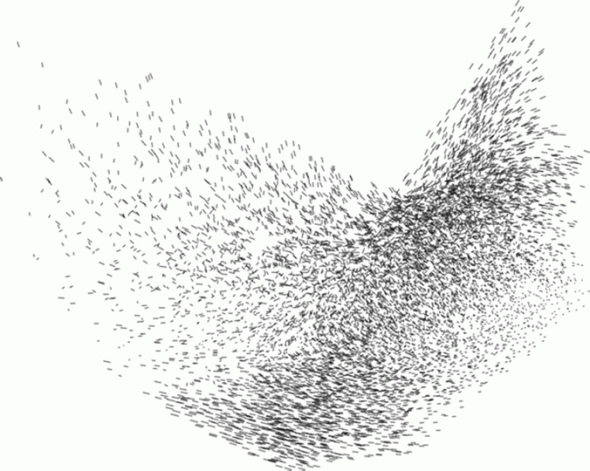
\includegraphics[width=5cm]{./img/swarm.png}}

\author[Grupo B4]{Felicia Burtscher, Frederik Eistrup, Jos\'{e} Senart\\  %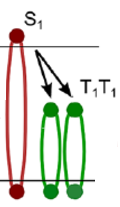
\includegraphics[width=0.15\columnwidth]{../img/SF_linda.pdf}\\
%\includegraphics[width=0.15\columnwidth]{../img/LBIC_CELLO_fig5.png}\includegraphics[width=0.15\columnwidth]{../img/LBIC_CELLO_fig9.png}
} % Your name

%\vspace{10pt}
%\includegraphics[width=0.2\columnwidth]{../img/LBIC_CELLO_fig9.png}\\

%\textit{"The imagination of nature is far, far greater than the imagination of man."} 
%, Richard Feynman}
%\textit{"Not everything that counts can be counted, \\and not everything that can be counted counts"}\\ Albert Einstein}
\date{\today} 
\institute[FUB]{\vspace{-10pt}Freie Universität Berlin}
%	\centering
\begin{document}

\begin{frame}
\titlepage
\end{frame}

%\begin{frame}\footnotesize
%\frametitle{Índice} % Table of contents slide, comment this block out to remove it
%\tableofcontents % Throughout your presentation, if you choose to use \section{} and \subsection{} commands, these will automatically be printed on this slide as an overview of your presentation
%\normalsize
%\end{frame}

%----------------------------------------------------------------------------------------
%	PRESENTATION SLIDES
%----------------------------------------------------------------------------------------

\begin{frame}
  \frametitle{Presentation Overview}

  \begin{itemize}
  	\item Review past models (simple speed coupling, couzin model, vicsek model)
	\item Module 1: Effective leadership and decision-making in animal groups on the move (Couzin et al)
	\item Module 2: Self-Propelled Particles with Soft-Core Interactions: Patterns, Stability, and Collapse (D'Orsogna et al)
%	\item Quantification
  \end{itemize}


 % \end{multicols}
\end{frame}

%\begin{frame}
%  \frametitle{Review past models (simple speed coupling, couszin model, viszek model)}
%  
%  
%%  \texttt{
%%  Models available:\\
%%  'Simple speed coupling..................smpl'
%%  'Couzin model...........................czn'
%%  'Couzin-2 model.........................czn2'
%%  'Viscek model...........................vsck'
%%  'Mill model.............................mill'
%%}
%  
%\end{frame}


\begin{frame}
	\frametitle{Review past models (simple speed coupling, vicsek model, couzin model)}
	
\textbf{Simple speed coupling}: weighted speed

\hspace{1cm}

Particle adapts a fraction of its nearest neighbour's speed.

\end{frame}


\begin{frame}
	\frametitle{Review past models (simple speed coupling, vicsek model, couzin model)}
	
	\textbf{Vicsek model} \\
	
	
	\begin{itemize}
		\item introduce interaction zones: repulsion and alignment
		\item add noise
	\end{itemize}
	
\end{frame}


\begin{frame}
	\frametitle{Review past models: simple speed coupling, vicsek model, couzin model}
	
	\textbf{Couzin model}
	
	\begin{itemize}
		\item different zones of neighbourhoods: repulsion, orientation, attraction
%		\item 
	\end{itemize}
	
\begin{figure}
%	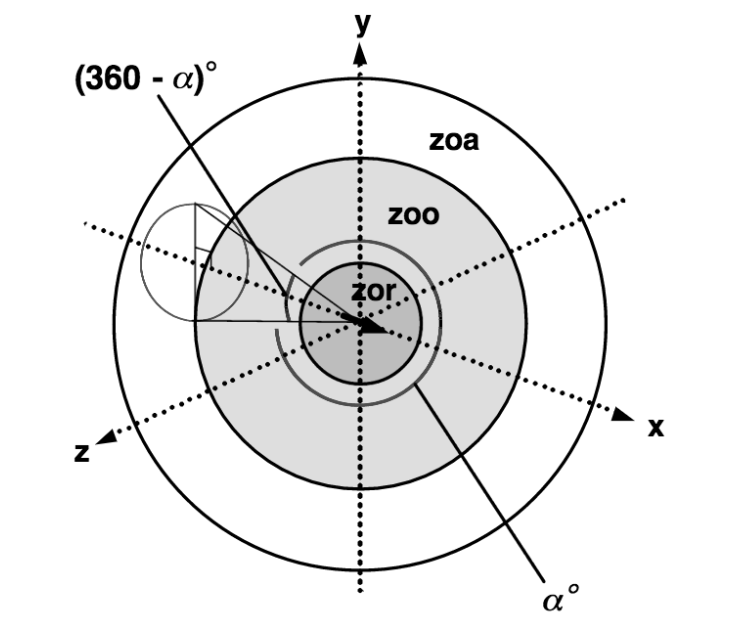
\includegraphics[width=.45\columnwidth, left]{./img/zones.png}
	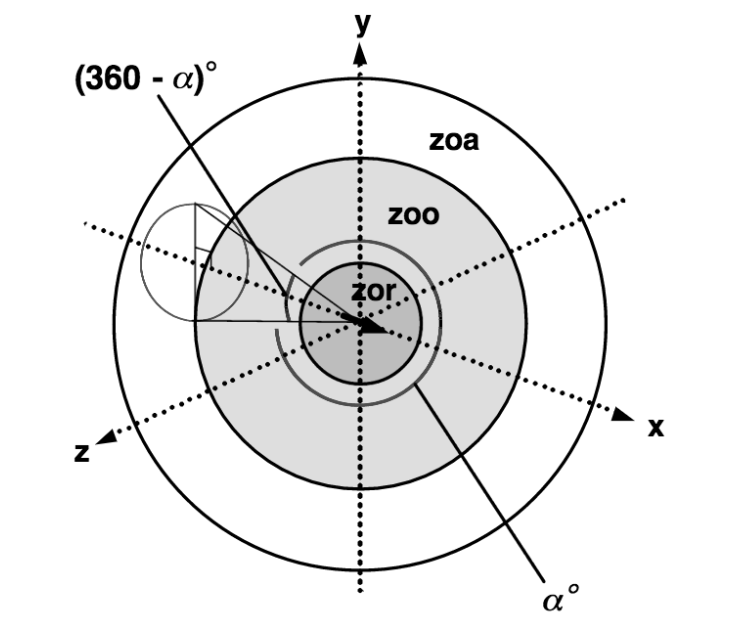
\includegraphics[width=.45\columnwidth]{./img/zones.png}
	\caption{Representation of an individual in the model centred at the origin: \textit{zor} = zone of repulsion, \textit{zoo} = zone of orientation, \textit{zoa} = zone of attraction. \( \alpha \) = field of perception}
	\label{zones}
\end{figure}

	
\end{frame}

%%%%---------------------------------------------------------------------------------------------

\begin{frame}
  \frametitle{Module 1: Effective leadership and decision-making in animal groups on the move (Couzin et al): \texttt{czn2}}
  
  We introduce a bias: orientation of \( \geq 1 \) particle (the "informed" one/ "scout") and merge orientation and attraction zone.
  
  
  \hspace{1cm}
  
 
 \textbf{THEORY} 
 
 \hspace{1cm}
 
\textbf{New parameters}: weight of bias, proportion of bias, group direction

\textbf{Goal:} Which parameter sets give a nice group movement, and how does the behaviour change when we change the parameters?

\hspace{1cm}

update of \( d_{i} \) in each zone: \\
\begin{figure}
	\begin{tabular}{cc}
		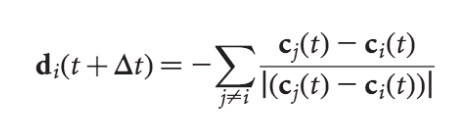
\includegraphics[width=35mm]{./img/eq1.png} &   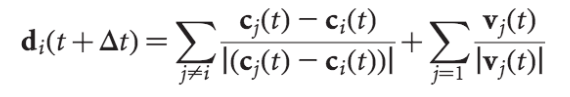
\includegraphics[width=40mm]{./img/eq2.png} \\
		%		(a) first & (b) second \\[6pt]
		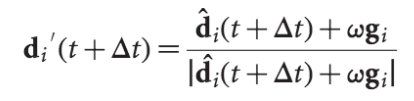
\includegraphics[width=30mm]{./img/eq3.png} \\
%		(d) fourth \\[6pt]
%		\multicolumn{2}{c}
%		{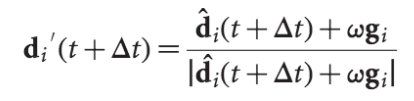
\includegraphics[width=40mm]{./img/eq3.png} }\\
		%		\multicolumn{2}{c}{(e) fifth}
	\end{tabular}
\end{figure}

\end{frame}


%\begin{frame}
%	\frametitle{Module 1: Effective leadership and decision-making in animal groups on the move (Couzin et al): \texttt{czn2}}
%	
%	\textbf{METHOD} 
%	
%	\hspace{1}
%	
%	\begin{itemize}
%		\item Explicit Euler method: \( v_{t+1}= v_{t} + \Delta t \cdot f(t_{n}, v_{t})  \)
%		\item How \( d \) is updated in each zone: see paper
%	\end{itemize}
%	
%	
%\end{frame}


%%%%------Senart's part------%%%%
\begin{frame}
	\frametitle{Module 1: Effective leadership and decision-making in animal groups on the move (Couzin et al): \texttt{czn2}}
	
	\textbf{IMPLEMENTATION} 
	
	\hspace{1cm}
	
	\begin{itemize}
		\item periodic boundary conditions
		\item virtual interaction of agents
		\item explicit Euler method: \( v_{n+1}= v_{n} + \tau \cdot f(t_{n}, v_{n})  \)
	\end{itemize}
	
	
\end{frame}


\begin{frame}
	\frametitle{Module 1: Effective leadership and decision-making in animal groups on the move (Couzin et al): \texttt{czn2}}
	
	\textbf{SIMULATION} on specific parameter set 
	
	
\end{frame}


\begin{frame}
	\frametitle{Module 1: Effective leadership and decision-making in animal groups on the move (Couzin et al): \texttt{czn2}}
	
	\textbf{QUANTIFICATION} 

	\hspace{1cm}
	
	\begin{itemize}
		\item Accuracy
		\item Group elongation
		\item Two scouts
	\end{itemize}
	
\end{frame}


\begin{frame}
	\frametitle{Module 1: Effective leadership and decision-making in animal groups on the move (Couzin et al): \texttt{czn2}}
	
	\textbf{SIMULATION} optimised
	
\end{frame}


%\begin{frame}
%	\frametitle{Paper 1: Effective leadership and decision-making in animal groups on the move (Couzin et al): \texttt{czn2}}
%	
%	\textbf{Bias, which parameter we control, show simulation gif}
%	
%\end{frame}



%%%%---------------------------------------------------------------------------------------------


%%%%------Felicia's part------%%%%
\begin{frame}
  \frametitle{Module 2: Self-Propelled Particles with Soft-Core Interactions: Patterns, Stability, and Collapse (D'Orsogna et al)}
  
  \textbf{Motivation}: Simulate swarming of multiagent systems in order to understand the operating principles of natural swarms, e.g. swarming behaviour of \textit{M. xanthus} cells. \\ 
  
  
  \begin{figure}
  		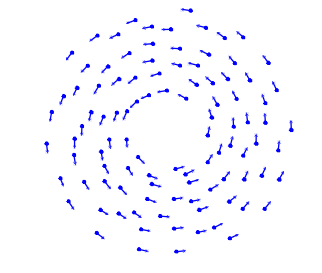
\includegraphics[width=0.18\columnwidth]{./img/mill.png}
  		\label{mill}
  \end{figure}


%\hspace{3}

  We choose a \textbf{kinetic theory} based approach.\\

\hspace{3cm}

  The model traits are:
  \begin{itemize}
  	\item self-propulsion
  	\item friction 
  	\item interaction between particles: repulsion and attraction
  \end{itemize}
 % as we will see this leads to various morphologies, e.f. flocks, rotating mills, rings and clumps.
 
%\small A kinetic theory based approach for swarming systems of self-propelled discrete particles. \\
%
% Individuals driven by self-propelling forces and pairwise attractive and repulsive interactions lead to various morphologies, e.f. flocks, rotating mills, rings and clumps. \\
%  We can \\
%  - average in direction or velocity \\
%  - consider different zones of interaction and averaging (see Couzin et al)

\end{frame}

\begin{frame}
  \frametitle{Module 2: Self-Propelled Particles with Soft-Core Interactions: Patterns, Stability, and Collapse (D'Orsogna et al)}
	
%	  
%	  But: As N=#particles grows, it becomes increasingly difficult to follows the dynamics of each individual agent. Therefore, we choose a continuous approach where particles are represented by a density field. \\
	  
	%\textbf{Discrete model}: \\ \\
	Consider \( N \) interacting, self-propelled particles governed by the following equations of motion
	
	
%	\begin{equation} \label{eqOfMotion}
%	\begin{split}
%    & \frac{\partial \vec{x_{i}}}{\partial t} = \vec{v_{i}} \\
%	m & \frac{\partial \vec{v_{i}}}{\partial t} = (\alpha - \beta |\vec{v_{i}}|^{2}) \vec{v_{i}} - \vec{\nabla_{i}} U(\vec{x_{i}})
%	\end{split}
%	\end{equation}
	
	
\begin{equation}
		\frac{d\vec{x_{i}}}{d t} = \vec{v_{i}}
\end{equation}

\begin{equation}
		    F = m  \frac{d\vec{v_{i}}}{d t} = (\textcolor{red}{\alpha}v- \textcolor{red}{\beta} |\vec{v_{i}}|^{2}) \vec{v_{i}} - \textcolor{red}{\vec{\nabla_{i}} U(\vec{x_{i}})}
\end{equation}

	
	where \( U \) is a pairwise interaction potential and \( \alpha, \beta > 0\) are values for propulsion and friction forces.\\

\end{frame}


\begin{frame}
  \frametitle{Module 2: Self-Propelled Particles with Soft-Core Interactions: Patterns, Stability, and Collapse (D'Orsogna et al)}
	

For \( U \) we choose the \textit{Morse potential} %which is a common choice for interacting swarming systems

\begin{equation} \label{morsePotential}
U(\vec{x_{i}}) = \sum_{j \neq i}^{} [ \underbrace{-C_{a} e^{-| \vec{x_{i}} - \vec{x_{j}} | / l_{a}}}_{\text{attraction}} + \underbrace{C_{r}e^{-|\vec{x_{i}}-\vec{x_{j}}|/l_{r}}}_{\text{repulsion}} ]
\end{equation}
where \( C_{a}\), \( C_{r}\) denote attractive and repulsive strengths and \( l_{a}\), \( l_{r}\) their respective length scales.


\begin{figure}
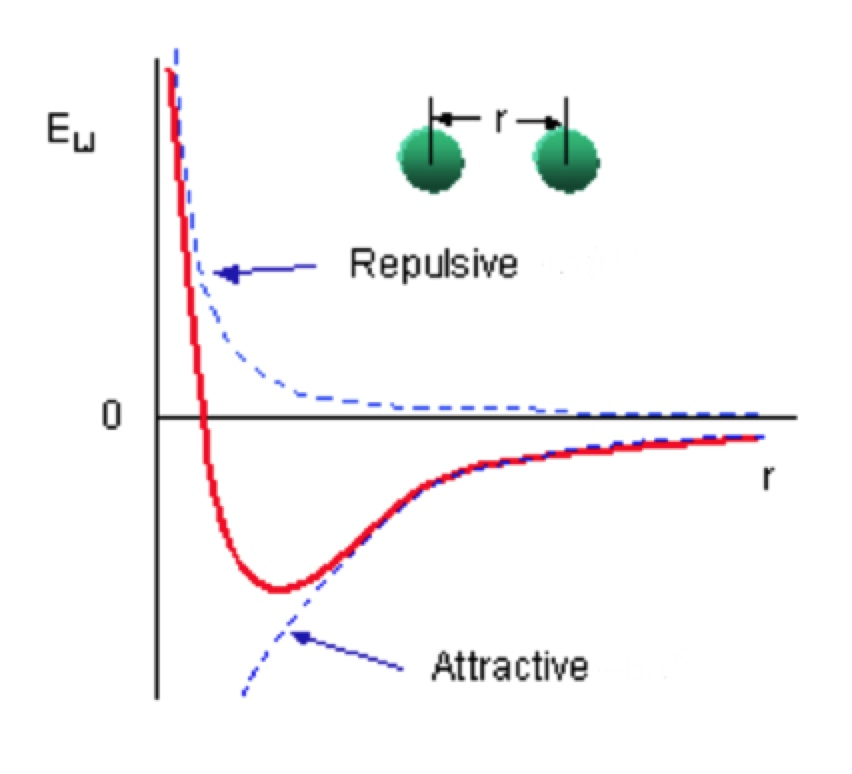
\includegraphics[width=.4\columnwidth]{./img/Morsepotential.jpg}
%\caption{Plot of the Morse potential}
\label{morsepotential}
\end{figure}

\end{frame}


%%%%---------------------------------------------------------------------------------------------
%%%%------Fred's part------%%%%
\begin{frame}
  \frametitle{Module 2: Self-Propelled Particles with Soft-Core Interactions: Patterns, Stability, and Collapse (D'Orsogna et al)}
	
	\textbf{IMPLEMENTATION}
	
	\begin{itemize}
		\item rigid boundary conditions
		\item no virtual interactions
		\item initial conditions of random distribution
		\item explicit Euler method to solve the ODEs
	\end{itemize}
	

\end{frame}


\begin{frame}
	\frametitle{Module 2: Self-Propelled Particles with Soft-Core Interactions: Patterns, Stability, and Collapse (D'Orsogna et al)}
	
	\textbf{SIMULATION}
	
	

	
\end{frame}


\begin{frame}
	\frametitle{Module 2: Self-Propelled Particles with Soft-Core Interactions: Patterns, Stability, and Collapse (D'Orsogna et al)}
	
	%	\textbf{Region simulation}
	%	
	%	INSERT simulation of different regions
	
	\begin{figure}[H]
		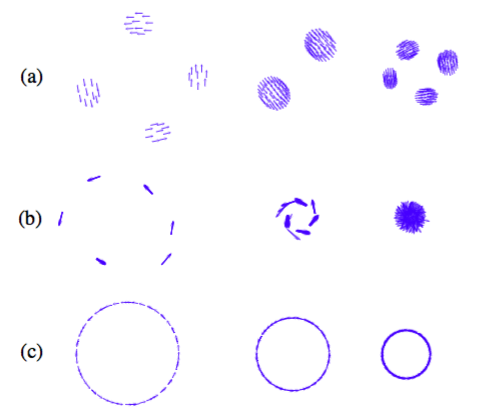
\includegraphics[width=.6\columnwidth]{./img/ClumpsRing.png}
		\caption{Catastrophic geometry. \\(a) Clumps. (b) Ring Clumping. (c) Rings.}
		\label{clumps}
	\end{figure}
	
\end{frame}



\begin{frame}
  \frametitle{Module 2: Self-Propelled Particles with Soft-Core Interactions: Patterns, Stability, and Collapse (D'Orsogna et al)}
	
%	\textbf{Quantification}
	
	\begin{figure}[H]
		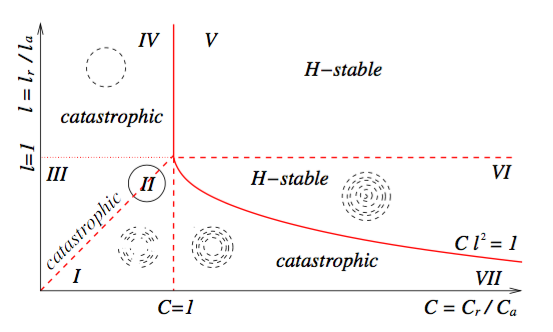
\includegraphics[width=.9\columnwidth]{./img/H-stabilityPhaseDiagram.png}
		\caption{H-stability phase diagram of the Morse potential}
		\label{hstability}
	\end{figure}
	
\end{frame}




\begin{frame}
  \frametitle{Module 2: Self-Propelled Particles with Soft-Core Interactions: Patterns, Stability, and Collapse (D'Orsogna et al)}
	
	
	Simulations: Region I, Region IV, Region VI, Region VII 
%	%	\textbf{Region simulation}
%	%	
%	%	INSERT simulation of different regions
%	
%	\begin{figure}[H]
%		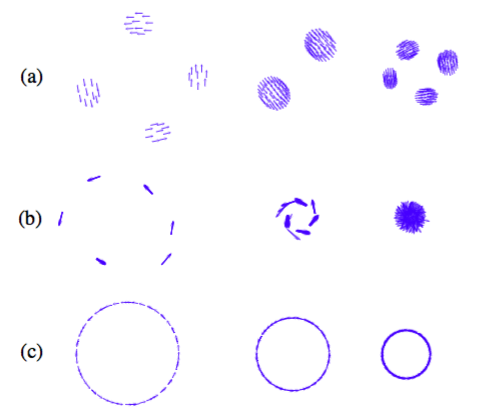
\includegraphics[width=.65\columnwidth]{./img/ClumpsRing.png}
%		\caption{Catastrophic geometry. \\(a) Clumps. (b) Ring Clumping. (c) Rings.}
%		\label{clumps}
%	\end{figure}
	
\end{frame}

% maybe: INTERESTING Trend of N: As N increases we get a smaller radius
%\begin{frame}
%  \frametitle{Module 2: Self-Propelled Particles with Soft-Core Interactions: Patterns, Stability, and Collapse (D'Orsogna et al)}
%	
%	\textbf{Simulation of catastrophic region VII}
%	
%	\begin{figure}[H]
%		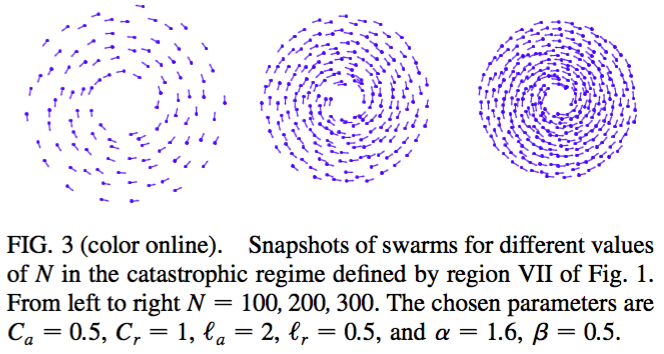
\includegraphics[width=1.\columnwidth]{./img/snapshots.png}
%		%\caption{snapshots of farms for different values of \( N \) in region VII. }
%		\label{snapshots}
%	\end{figure}
%	
%
%\end{frame}


%\begin{frame}
%	\frametitle{Quantification \texttt{mill}}
%	
%	\begin{figure}[H]
%		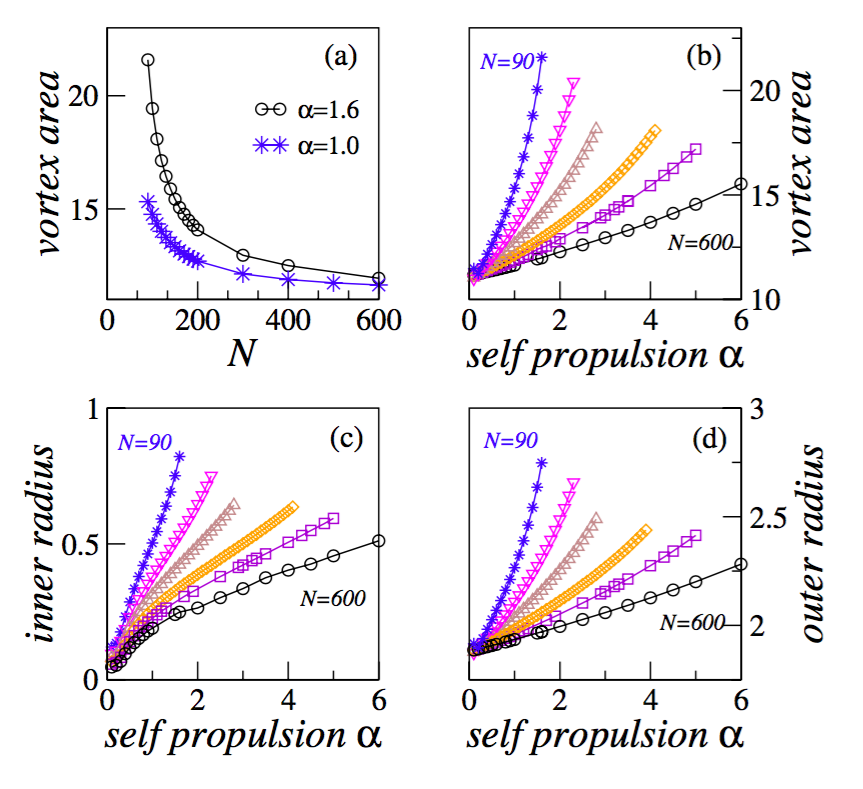
\includegraphics[width=.7 \columnwidth]{./img/vortexScaling.png}
%		\caption{Vortex scaling for the catastrophic Morse potential.}
%		\label{vortexScaling}
%	\end{figure}
%	
%
%\end{frame}


\begin{frame}
  \frametitle{Module 2: Self-Propelled Particles with Soft-Core Interactions: Patterns, Stability, and Collapse (D'Orsogna et al)}
	
	\textbf{QUANTIFICATION} \small (Goals of Observation) \normalsize
	
	\begin{itemize}
		\item Parameter Sets for different Stability Regions
		\item Confirming Ring formation: \\
			- \( R_{max}, R_{mean}, R_{min} \) converge to same value \\
			- \( v_{radial} \to 0 \) and \( v_{tangential} \to | v_{i} |  \) for \( t \to \infty \)
	\end{itemize}
\end{frame}


\begin{frame}
	\frametitle{Quantification \texttt{mill} \small (Region II: Convergence to Ring)} \normalsize
	\begin{figure}[H]
		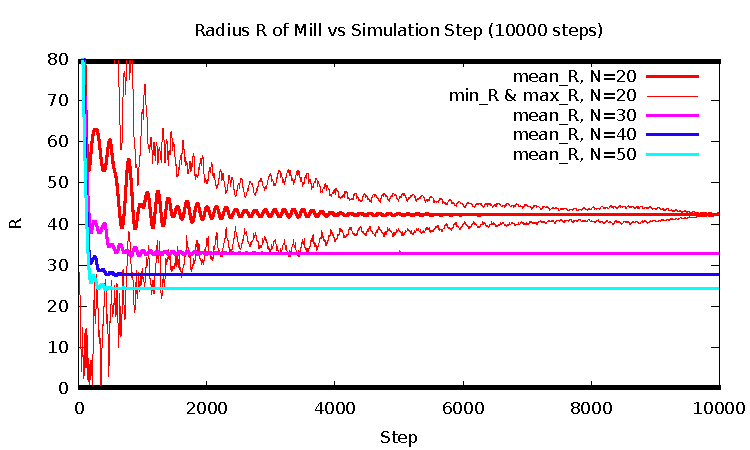
\includegraphics[width=1. \columnwidth]{../plots/mill_II_radius_dt_allN.pdf}
	\end{figure}	
\end{frame}


\begin{frame}
	\frametitle{Quantification \texttt{mill} \small (Region II: Convergence to Ring)} \normalsize
	\begin{figure}[H]
		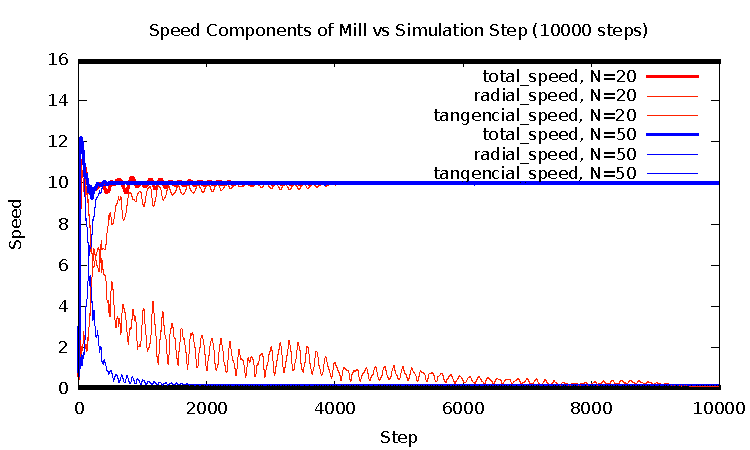
\includegraphics[width=1. \columnwidth]{../plots/mill_II_speeds_dt_allN.pdf}
	\end{figure}	
\end{frame}

\begin{frame}
	\frametitle{Quantification \texttt{mill} \small (Goals of Observation)} \normalsize
	\begin{itemize}
		\item Parameter Sets for different Stability Regions
		\item Confirming Ring formation: \\
			- \( R_{max}, R_{mean}, R_{min} \) converge to same value \\
			- \( v_{radial} \to 0 \) and \( v_{tangential} \to | v_{i} |  \) for \( t \to \infty \)
		\item  \( R \propto \frac{\alpha m}{\beta}\) \small (from  \( F_{centrifugal} = F_{centripetal} \)) \normalsize
	\end{itemize}
\end{frame}



\begin{frame}
	\frametitle{Quantification \texttt{mill}  \small (Region II: Effect on Radius of Ring)} \normalsize
\begin{figure}[H]
	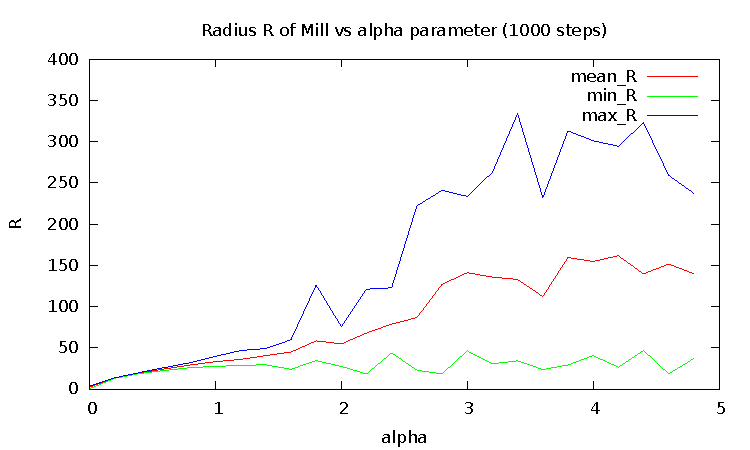
\includegraphics[width=1. \columnwidth]{../plots/mill_II_radius_alpha_1000.pdf}
\end{figure}
\end{frame}

\begin{frame}
	\frametitle{Quantification \texttt{mill} \small (Region II: Effect on Radius of Ring)}
	\begin{figure}[H]
		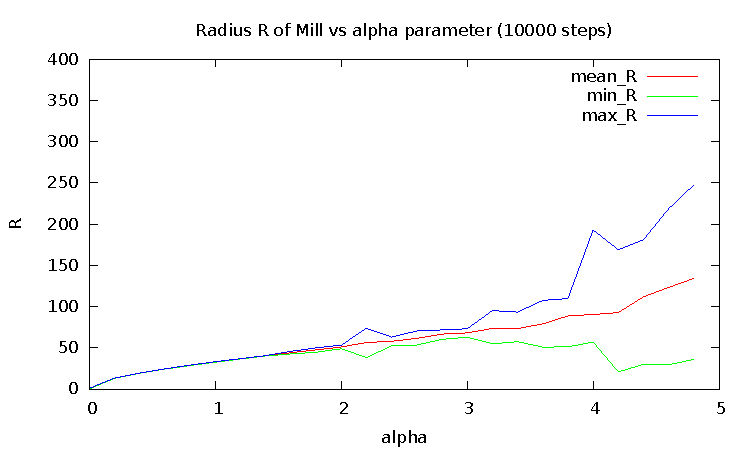
\includegraphics[width=1. \columnwidth]{../plots/mill_II_radius_alpha_10000.pdf}
	\end{figure}
\end{frame}

\begin{frame}
	\frametitle{Quantification \texttt{mill} \small (Region II: Effect on Radius of Ring)}
	\begin{figure}[H]
		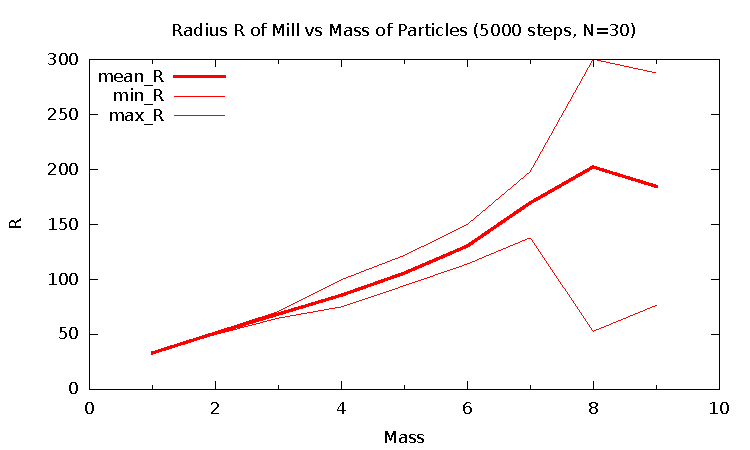
\includegraphics[width=1. \columnwidth]{../plots/mill_II_radius_mass.pdf}
	\end{figure}
\end{frame}


\begin{frame}
	\frametitle{Quantification \texttt{mill} \small (Region II: Effect on Radius of Ring )} \normalsize	
	\begin{figure}[H]
		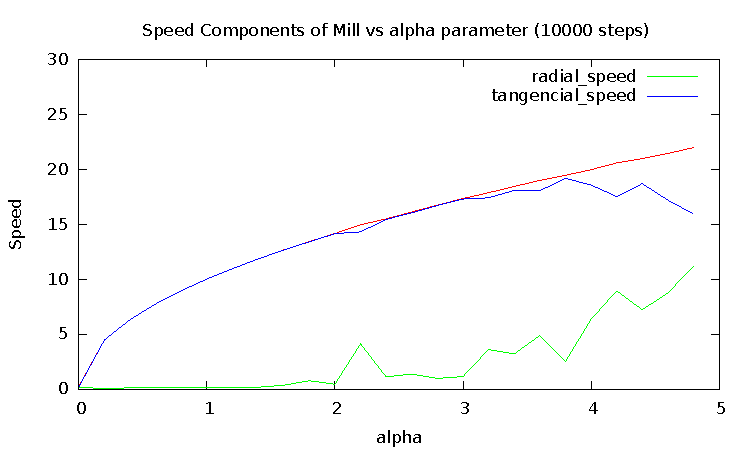
\includegraphics[width=1. \columnwidth]{../plots/mill_II_speeds_alpha_10000.pdf}
	\end{figure}	
\end{frame}





\begin{frame}
	\frametitle{Quantification \texttt{mill} \small (Goals of Observation)} \normalsize
	\begin{itemize}
		\item Parameter Sets for different Stability Regions
		\item Confirming Ring formation: \\
			- \( R_{max}, R_{mean}, R_{min} \) converge to same value \\
			- \( v_{radial} \to 0 \) and \( v_{tangential} \to | v_{i} |  \) for \( t \to \infty \)
		\item  \( R \propto \frac{\alpha m}{\beta}\) \small (from  \( F_{centrifugal} = F_{centripetal} \)) \normalsize
		\item \( |\vec{v}|^{2} \xrightarrow{t \to \infty}  \alpha / \beta \) \small(at steady state \( (\alpha - |\vec{v}|^2 \beta ) \vec{v} = 0 \)) 
\normalsize
	\end{itemize}
\end{frame}


%\begin{frame}
%	\frametitle{Quantification \texttt{mill} \small (Region II: Influence of \( \alpha \) )} \normalsize
%	\begin{figure}[H]
%		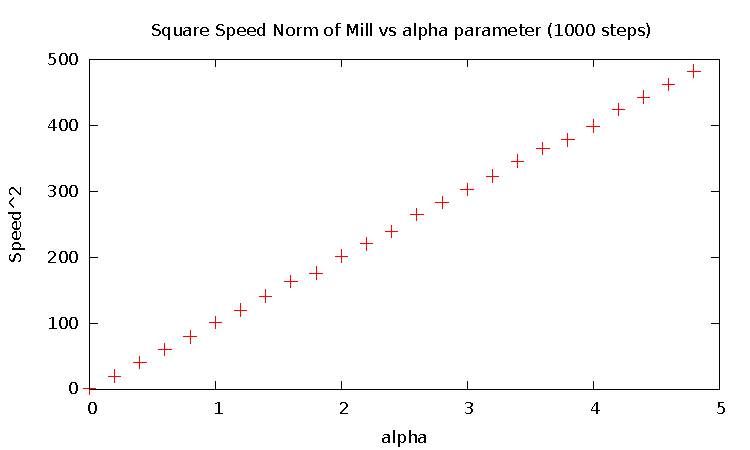
\includegraphics[width=1. \columnwidth]{../plots/mill_II_square_alpha_1000.pdf}
%	\end{figure}
%\end{frame}


\begin{frame}
	\frametitle{Quantification \texttt{mill} \small (Region II: Influence of \( \alpha \) )} \normalsize
	\begin{figure}[H]
		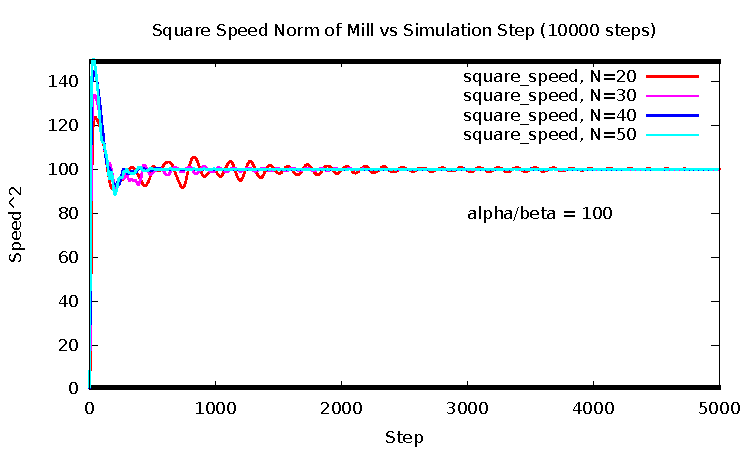
\includegraphics[width=1. \columnwidth]{../plots/mill_II_square_dt_allN.pdf}
	\end{figure}	
\end{frame}

\begin{frame}
	\frametitle{Quantification \texttt{mill} \small (Region II: Influence of \( \alpha \) )} \normalsize
	\begin{figure}[H]
		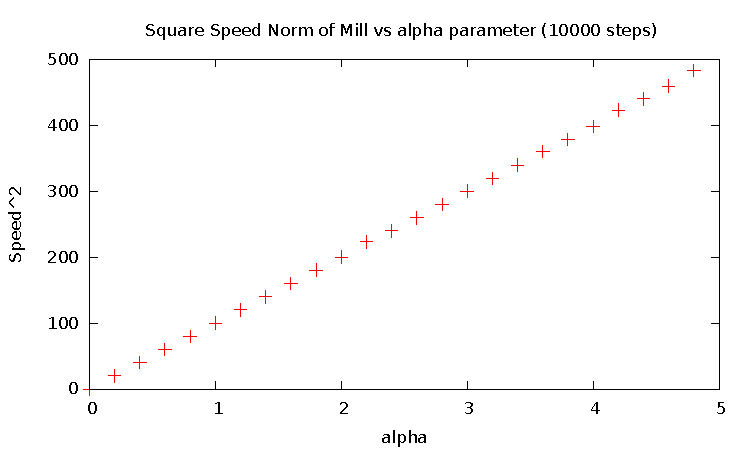
\includegraphics[width=1. \columnwidth]{../plots/mill_II_square_alpha_10000.pdf}
	\end{figure}
\end{frame}





\begin{frame}
	\frametitle{Quantification \texttt{mill} \small (Goals of Observation)} \normalsize
	\begin{itemize}
		\item Parameter Sets for different Stability Regions
		\item Confirming Ring formation: \\
			- \( R_{max}, R_{mean}, R_{min} \) converge to same value \\
			- \( v_{radial} \to 0 \) and \( v_{tangential} \to | v_{i} |  \) for \( t \to \infty \)
		\item  \( R \propto \frac{\alpha m}{\beta}\) \small (from  \( F_{centrifugal} = F_{centripetal} \)) \normalsize
		\item \( |\vec{v}|^{2} \xrightarrow{t \to \infty}  \alpha / \beta \) \small(at steady state \( (\alpha - |\vec{v}|^2 \beta ) \vec{v} = 0 \)) 
\normalsize
		\item influence of increasing \( N \)
		%	\item (trend of N, e.g. in simulation of region VII)
	\end{itemize}
\end{frame}


\begin{frame}
	\frametitle{Quantification \texttt{mill} \small (Region II: influence of N)} \normalsize
	\begin{figure}[H]
		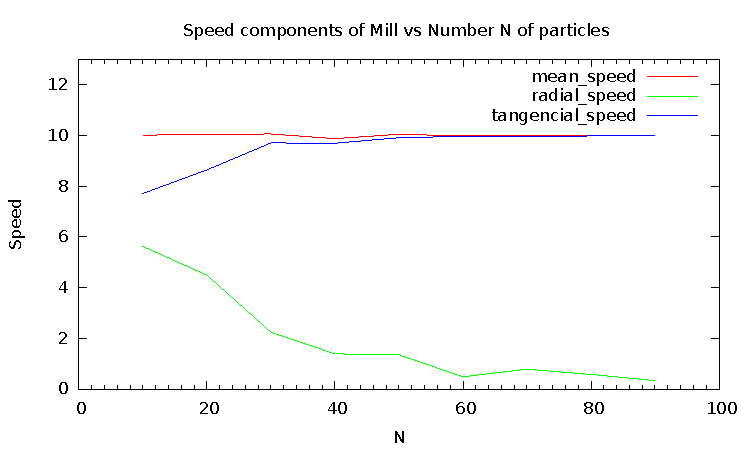
\includegraphics[width=1. \columnwidth]{../plots/mill_II_speeds_N.pdf}
	\end{figure}	
\end{frame}


\begin{frame}
	\frametitle{Quantification \texttt{mill} \small (Region II: influence of N)} \normalsize
	
\begin{figure}[H]
		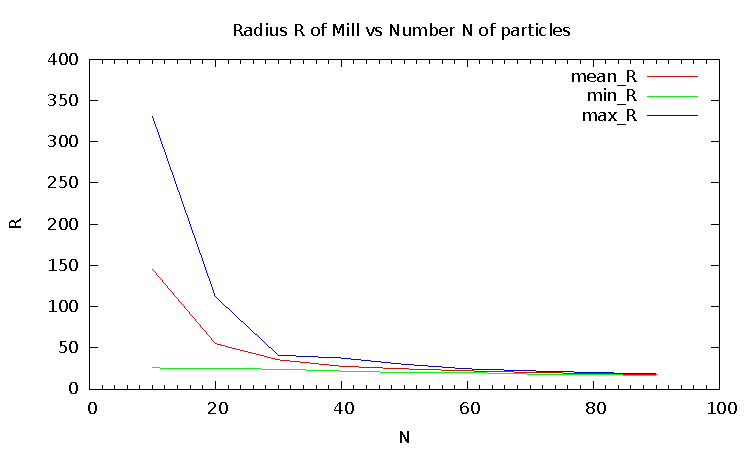
\includegraphics[width=1. \columnwidth]{../plots/mill_II_radius_N.pdf}
\end{figure}

\end{frame}


\begin{frame}
	\frametitle{Quantification \texttt{mill} \small ( Region VII: Torus Ring)} \normalsize
	
\begin{figure}[H]
		\includegraphics[width=0.7 \columnwidth]{../plots/mill_VII_speeds_radius_N_d.pdf}
\end{figure}

\end{frame}


\end{document}


